\documentclass[a4paper,12pt]{article}
\usepackage{amssymb}
\usepackage{amsmath}
\usepackage{xcolor,color}
\usepackage{tikz}
\usetikzlibrary{shapes.geometric,positioning,decorations.pathreplacing,decorations.pathmorphing,patterns,decorations.markings}

\begin{document}

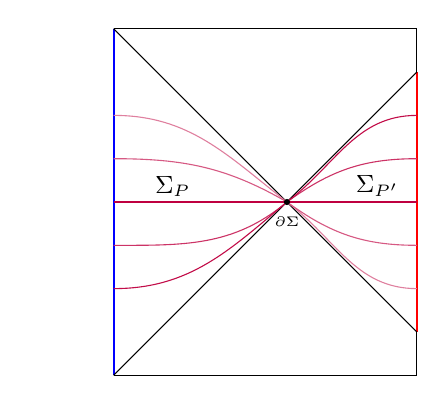
\begin{tikzpicture}[scale=1.1]


\coordinate (A) at (-2,2.8) ;
\coordinate (B) at (-1.4,3.4);

\draw[thick,blue %,-<
](-2,0) --++(0,2.2);
\draw[thick,blue] (-2,2) --++(0,2) ;
\draw[thick,red %, ->
](1.5,0.5) --++(0,1.5);
\draw[thick,red] (1.5,2) --++(0,1.5) ;
\draw (1.5,3.5)--++(0,0.5);
\draw (1.5,0)--++(0,0.5);
\draw (-2,0)--++(3.5,3.5);
\draw (+1.5,0.5)--++(-3.5,3.5);
\draw (-2,0) -++(3.5,0) ;%--++(-2,2);
\draw (-2,4)--++(3.5,0);



\draw[purple,thick] (+1.5,2.0) node[above=-1.8pt]{\hskip-1cm\small $\color{black} \Sigma_{P'}$} --(-2.0,2.0) node[above=-1.8pt]{\hskip1.5cm\small $\color{black} \Sigma_{P}$} ;

\coordinate (C) at (0.0,2.0) ;


\draw[purple!50] (1.5,1.0)  to [out=180, in = -37]   (C) to  [out=142, in = 0]    (-2.0,3.0) ;

\draw[purple!65] (1.5,1.5)  to [out=180, in = -36]  (C) to  [out=150, in = 0]    (-2.0,2.5) ;

\draw[purple!80] (1.5,2.5)  to [out=180, in = 36]  (C) to  [out=220, in = 0]    (-2.0,1.5) ;

\draw[purple!95] (1.5,3.0)  to [out=180, in = 37]  (C) to  [out=220, in = 0]    (-2.0,1.0) ;
\filldraw[black] (0,2) circle (0.8pt) node[below=2pt] {\tiny $\partial \Sigma$};


\end{tikzpicture}

\end{document}